The theme of the ``Snowmass on the Mississippi'' exercise can be simply summed up as ``How do we find New Physics?''. The Intensity Frontier answer evokes the power and reach of virtual processes in both finding evidence for New Physics and constraining its properties. Experiments in the lepton sector of the Intensity Frontier, by searching for rare decay processes involving lepton flavor violation and $C\!P$-violation, and by making precision measurements of quantities whose value is extremely well-predicted in the Standard Model, can advance our understanding of the most basic features of the Standard Model for which we currently have no rationale. Why are there three lepton families? Since lepton flavor conservation is violated in the neutrino sector, is it violated in the charged lepton sector as well? Why are the patterns of lepton and quark flavor mixing so different?

 Charged leptons are unique in several ways:
\begin{itemize}
\item
They directly probe the couplings of new particles to leptons.  This is unique in that the current energy frontier machine, the 
CERN LHC, is a hadron
collider. It is very effective at probing the quark sector, but
is significantly more limited in the lepton sector.
\item
Very
precise measurements  and sensitive searches can be made at a level that is difficult to achieve in
other sectors.
\item
They can be studied using a diverse set of independent
processes. The combination of these studies can provide additional
insights into the structure of the lepton sector.
\item
Hadronic uncertainties in the Standard Model predictions are either insignificant, or in the case of muon $g-2$, are obtained using independent data sets and estimates from theory
%Hadronic uncertainties in the Standard Model predictions are either insignificant, or in the case of muon $g\!-\!2$, are controlled using independent data sets.
\item
There are  many cases, in particular charged lepton flavor violation (CLFV), where any signal would be an indisputable discovery of physics beyond the Standard Model (henceforth BSM physics).
\end{itemize}

There are important charged lepton observables that are best studied using electrons, most notably the electron electric dipole moment (EDM).  In most cases, these experiments are performed using outer-shell or shared electrons in either atoms or molecules.  These topics are covered in detail by the Nucleons/Nuclei/Atoms working group; we refer the reader to that chapter of these proceedings.

The program of studies of charged leptons is diverse, encompassing highly optimized, single-purpose experiments that focus on near-forbidden interactions of muons and multi-purpose experiments that take advantage of the large $\tau$-pair production cross section at $B$ or $\tau$/charm factories .
Very large
improvements in sensitivity are possible in the near future; even larger sensitivity gains can be made at Project X.  New
experiments such as Mu2e can probe rare processes at rates four orders
of magnitude more sensitive than current bounds. At this level of sensitivity many models predict that there will be observations of SM-forbidden processes, not just limits. These 
improvements will be a significant part of the program to understand new short-distance dynamics or new ultra-weak interactions.

Aside from being an intergral part of the broader Intensity Frontier program, studies of the  charged lepton sector provide  a vital link to the Energy Frontier. In the same way that, taken together, the results of individual charged
lepton experiment are more sensitive to BSM physics, charged lepton sector results as a whole are more
powerful when considered in concert with other Intensity and Energy Frontier experiments.  In
particular, there are three domains in which such combined results are a
crucial probe of BSM physics.   First, since neutrinos and charged leptons form a 
natural doublet, one would expect any BSM effects
 in neutrinos to also be seen in sufficiently sensitive charged lepton experiments.  
 Second, any complete theory of 
 flavor generation and the observed matter-antimatter asymmetry of the universe must 
 relate flavor and $C\!P$ (or $T$) violation in the heavy quark, neutrino, and charged lepton sectors.  
 Third,  any theory that predicts new particles or interactions at the LHC must also account for the virtual effects of those particles on decays and interactions of charged leptons and heavy quarks.
Thus, the major expansion in the study of charged leptons now underway is a natural extension of the successful heavy quark, neutrino and energy frontier programs of the previous decades.

A fourth domain is the probe of new ultra-weak, low energy interactions, referred to collectively  as hidden or dark sectors.  Here, charged lepton experiments overlap  with a wide variety of
experiments at the Intensity, Cosmic, and Energy Frontiers.  A large
experimental program is now under way to directly probe for new
hidden sectors, particularly in regions of parameter space
consistent with the muon $g-2$ anomaly.  This program is covered
in detail in the ``New Light Weakly-Coupled Particles'' chapter of this report.

\begin{figure}[t!]
\begin{center}
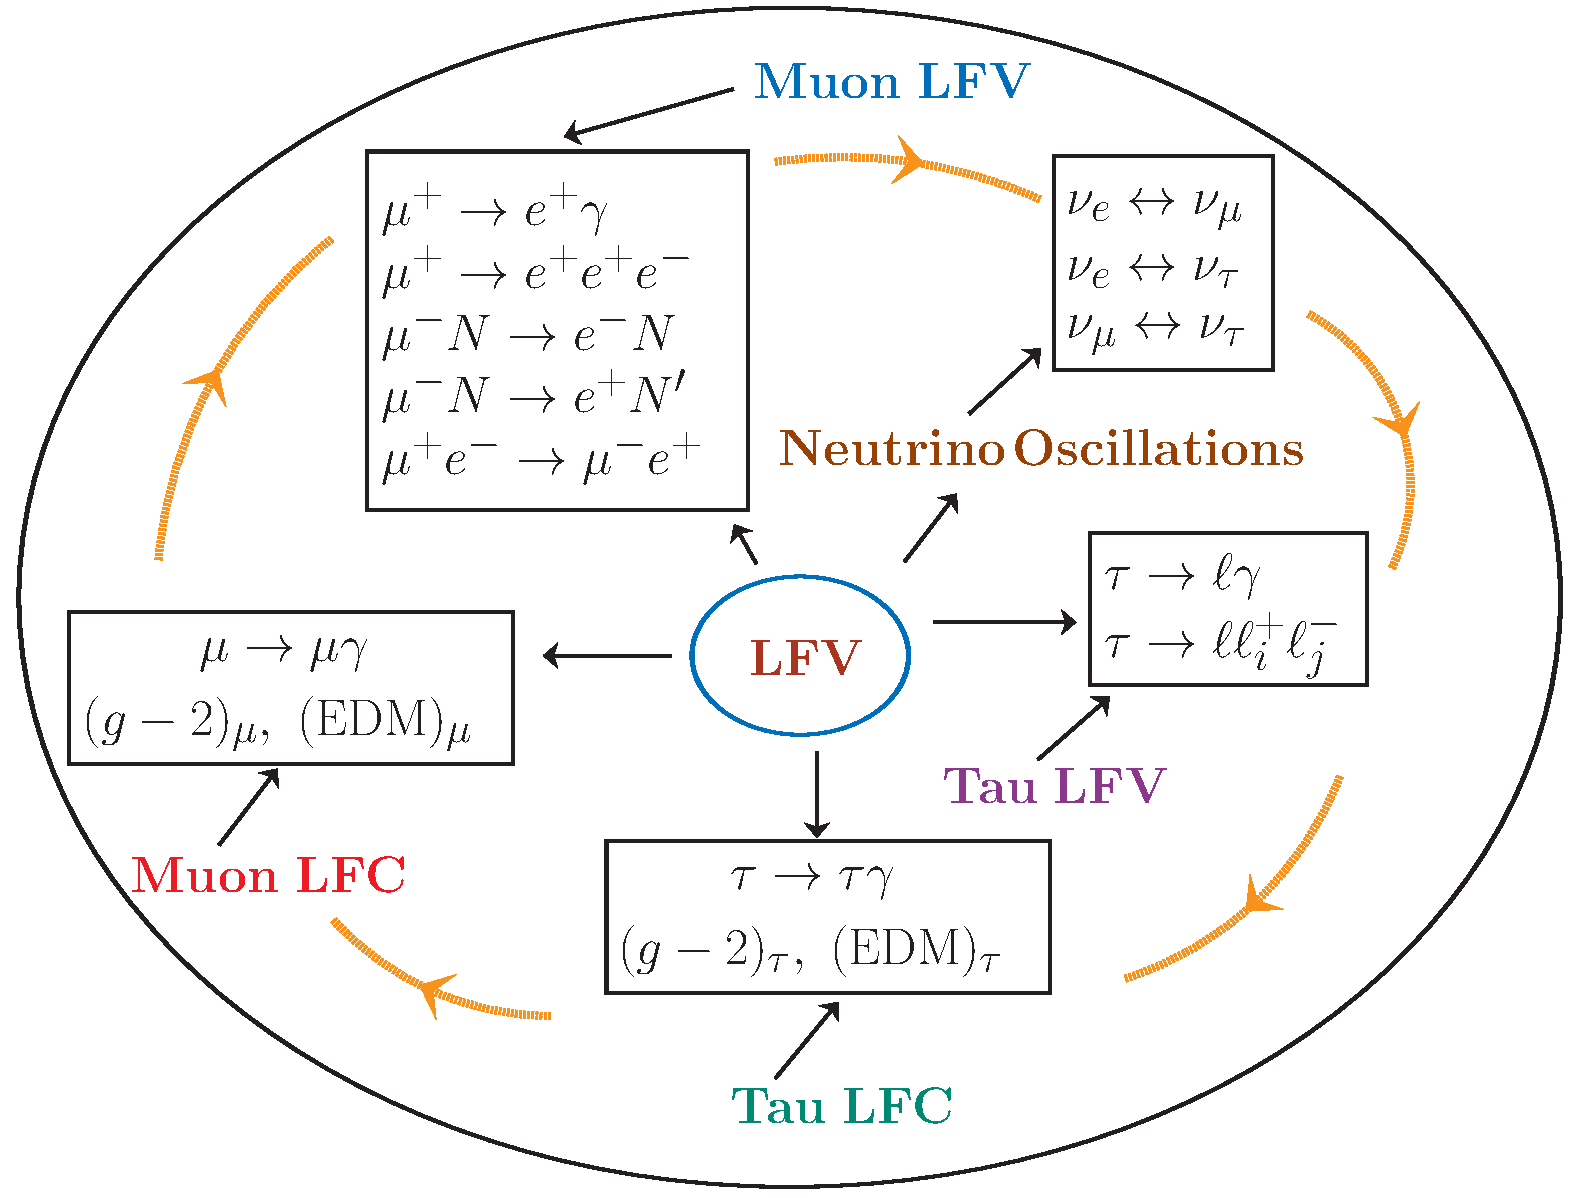
\includegraphics[width=10cm]{ChargedLeptons/Figures/chart.pdf}
\caption{\label{CL:chart}Interconnection between various lepton flavor violating and  lepton flavor conserving processes.}
\end{center}
\end{figure}

Fig. \ref{CL:chart} schematically depicts the interconnection between
various flavor-conserving and -violating processes in the lepton
sector.  In an underlying theory, neutrino flavor oscillations,
charged lepton flavor violation,  the anomalous magnetic moments, and permanent electric
dipole moments are all related.  Each experimental avenue we pursue allows us to uncover further attributes of the underlying theory. 

There are many important physical observables potentially sensitive to
BSM effects in charged lepton processes. Below, they are  split into  flavor violating observables and flavor conserving observables  such as $g-2$, EDMs, and parity violation measurements. Tau decays offer a unique opportunity to simultaneously study flavor-conserving, flavor-violating, $C\!P$-violating,  and $T$-violating effects and are discussed in
 their own section below.